\documentclass{article}
\usepackage[T1]{fontenc}
\usepackage[utf8]{inputenc}
\usepackage{lmodern}
\usepackage[T1]{fontenc}
\usepackage[utf8]{inputenc}
\usepackage{lmodern}
\usepackage[tmargin=1cm,lmargin=1cm]{geometry}
\usepackage{tikz}
\usepackage{pgfplots}
\pgfplotsset{compat=newest}
\usepackage{pgfplots}


\begin{document}
\section{Series: h}
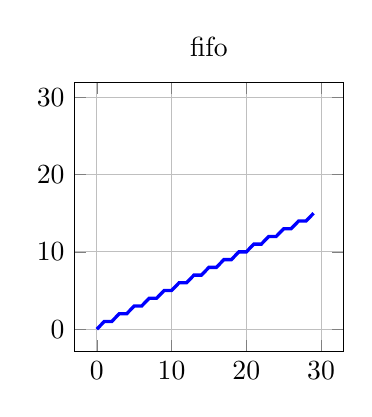
\begin{tikzpicture}
\begin{axis}[title=fifo, height=5cm, width=5cm, grid=major, xmin=({-}3.0), xmax=(33.0), ymin=({-}2.9), ymax=(31.9)]
\addplot[very thick,color=blue] coordinates {
(0,0)
(1,1)
(2,1)
(3,2)
(4,2)
(5,3)
(6,3)
(7,4)
(8,4)
(9,5)
(10,5)
(11,6)
(12,6)
(13,7)
(14,7)
(15,8)
(16,8)
(17,9)
(18,9)
(19,10)
(20,10)
(21,11)
(22,11)
(23,12)
(24,12)
(25,13)
(26,13)
(27,14)
(28,14)
(29,15)
};


\end{axis}
\end{tikzpicture}
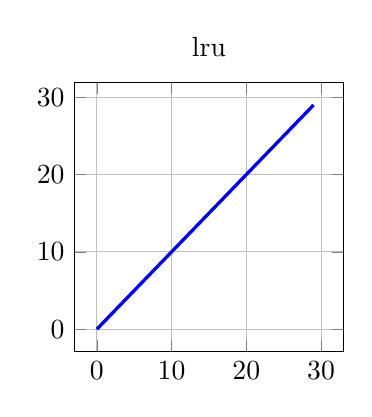
\begin{tikzpicture}
\begin{axis}[title=lru, height=5cm, width=5cm, grid=major, xmin=({-}3.0), xmax=(33.0), ymin=({-}2.9), ymax=(31.9)]
\addplot[very thick,color=blue] coordinates {
(0,0)
(1,1)
(2,2)
(3,3)
(4,4)
(5,5)
(6,6)
(7,7)
(8,8)
(9,9)
(10,10)
(11,11)
(12,12)
(13,13)
(14,14)
(15,15)
(16,16)
(17,17)
(18,18)
(19,19)
(20,20)
(21,21)
(22,22)
(23,23)
(24,24)
(25,25)
(26,26)
(27,27)
(28,28)
(29,29)
};


\end{axis}
\end{tikzpicture}
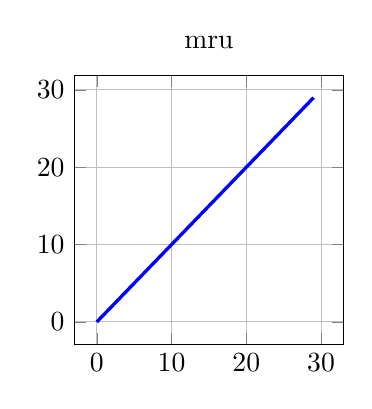
\begin{tikzpicture}
\begin{axis}[title=mru, height=5cm, width=5cm, grid=major, xmin=({-}3.0), xmax=(33.0), ymin=({-}2.9), ymax=(31.9)]
\addplot[very thick,color=blue] coordinates {
(0,0)
(1,1)
(2,2)
(3,3)
(4,4)
(5,5)
(6,6)
(7,7)
(8,8)
(9,9)
(10,10)
(11,11)
(12,12)
(13,13)
(14,14)
(15,15)
(16,16)
(17,17)
(18,18)
(19,19)
(20,20)
(21,21)
(22,22)
(23,23)
(24,24)
(25,25)
(26,26)
(27,27)
(28,28)
(29,29)
};


\end{axis}
\end{tikzpicture}
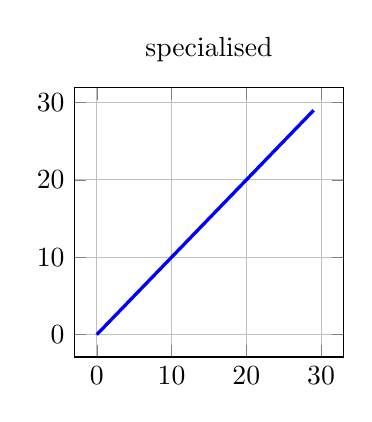
\begin{tikzpicture}
\begin{axis}[title=specialised, height=5cm, width=5cm, grid=major, xmin=({-}3.0), xmax=(33.0), ymin=({-}2.9), ymax=(31.9)]
\addplot[very thick,color=blue] coordinates {
(0,0)
(1,1)
(2,2)
(3,3)
(4,4)
(5,5)
(6,6)
(7,7)
(8,8)
(9,9)
(10,10)
(11,11)
(12,12)
(13,13)
(14,14)
(15,15)
(16,16)
(17,17)
(18,18)
(19,19)
(20,20)
(21,21)
(22,22)
(23,23)
(24,24)
(25,25)
(26,26)
(27,27)
(28,28)
(29,29)
};


\end{axis}
\end{tikzpicture}


\section{Series: math.log10(h / h + ncm + cm)}
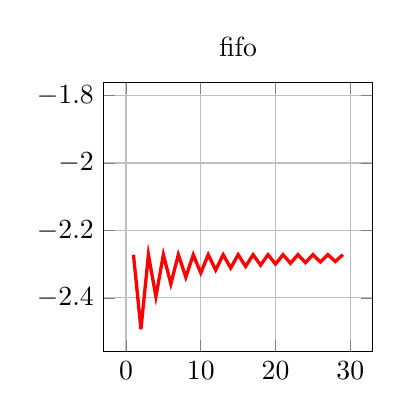
\begin{tikzpicture}
\begin{axis}[title=fifo, height=5cm, width=5cm, grid=major, xmin=({-}3.0), xmax=(33.0), ymin=({-}2.5593), ymax=({-}1.7614)]
\addplot[very thick,color=red] coordinates {
(1,-2.271841606536499)
(2,-2.4927603890268375)
(3,-2.271841606536499)
(4,-2.3961993470957363)
(5,-2.271841606536499)
(6,-2.3585693167727633)
(7,-2.271841606536499)
(8,-2.3384564936046046)
(9,-2.271841606536499)
(10,-2.325925955771466)
(11,-2.271841606536499)
(12,-2.317366791939507)
(13,-2.271841606536499)
(14,-2.3111481503830875)
(15,-2.271841606536499)
(16,-2.3064250275506875)
(17,-2.271841606536499)
(18,-2.302715643121607)
(19,-2.271841606536499)
(20,-2.299725153975637)
(21,-2.271841606536499)
(22,-2.2972629804204754)
(23,-2.271841606536499)
(24,-2.2952004520032574)
(25,-2.271841606536499)
(26,-2.2934475521638946)
(27,-2.271841606536499)
(28,-2.2919394147752556)
(29,-2.271841606536499)
};


\end{axis}
\end{tikzpicture}
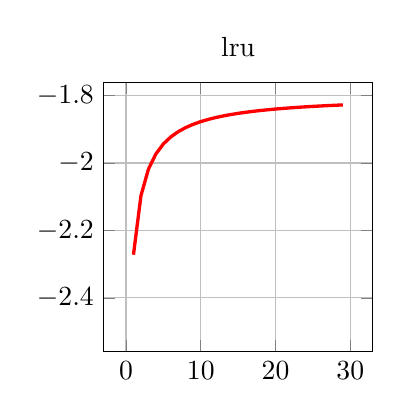
\begin{tikzpicture}
\begin{axis}[title=lru, height=5cm, width=5cm, grid=major, xmin=({-}3.0), xmax=(33.0), ymin=({-}2.5593), ymax=({-}1.7614)]
\addplot[very thick,color=red] coordinates {
(1,-2.271841606536499)
(2,-2.0969100130080562)
(3,-2.018423082826786)
(4,-1.9731278535996988)
(5,-1.9434945159061026)
(6,-1.9225524667613758)
(7,-1.9069504078051818)
(8,-1.8948696567452525)
(9,-1.8852355379348735)
(10,-1.877371345869774)
(11,-1.8708293713741904)
(12,-1.8653014261025438)
(13,-1.8605683404304916)
(14,-1.8564699450416706)
(15,-1.8528864461530967)
(16,-1.849726444196328)
(17,-1.8469189839058826)
(18,-1.844408136005944)
(19,-1.8421492166616982)
(20,-1.8401060944567578)
(21,-1.8382492363851182)
(22,-1.836554266470963)
(23,-1.835000886605694)
(24,-1.8335720576236982)
(25,-1.832253370197008)
(26,-1.8310325561052112)
(27,-1.8298991046335062)
(28,-1.8288439586198308)
(29,-1.827859271495562)
};


\end{axis}
\end{tikzpicture}
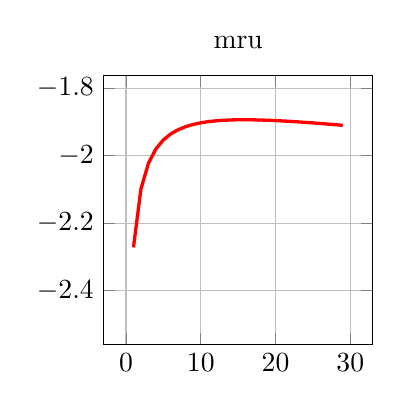
\begin{tikzpicture}
\begin{axis}[title=mru, height=5cm, width=5cm, grid=major, xmin=({-}3.0), xmax=(33.0), ymin=({-}2.5593), ymax=({-}1.7614)]
\addplot[very thick,color=red] coordinates {
(1,-2.271841606536499)
(2,-2.098643725817057)
(3,-2.0225658278987413)
(4,-1.9800033715837464)
(5,-1.9532763366673043)
(6,-1.9353392927102988)
(7,-1.9227995760038339)
(8,-1.9138138523837167)
(9,-1.907291901419713)
(10,-1.9025467793139914)
(11,-1.8991237997743422)
(12,-1.896709890354168)
(13,-1.8950823897800735)
(14,-1.894078591896473)
(15,-1.8935768378559144)
(16,-1.893484346218486)
(17,-1.893729134096401)
(18,-1.8942545086510418)
(19,-1.895015222183821)
(20,-1.8959747323590646)
(21,-1.8971032136854176)
(22,-1.898376090295125)
(23,-1.8997729371806873)
(24,-1.9012766462284754)
(25,-1.9028727854460794)
(26,-1.904549101094636)
(27,-1.906295126867155)
(28,-1.9081018741851592)
(29,-1.9099615846253677)
};


\end{axis}
\end{tikzpicture}
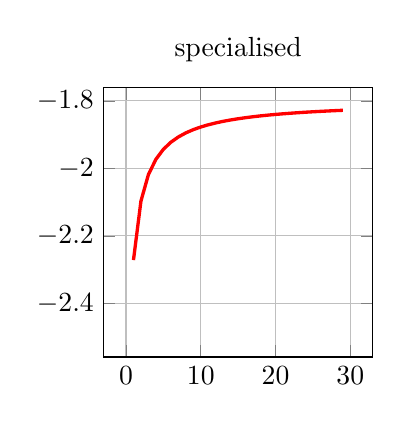
\begin{tikzpicture}
\begin{axis}[title=specialised, height=5cm, width=5cm, grid=major, xmin=({-}3.0), xmax=(33.0), ymin=({-}2.5593), ymax=({-}1.7614)]
\addplot[very thick,color=red] coordinates {
(1,-2.271841606536499)
(2,-2.0969100130080562)
(3,-2.018423082826786)
(4,-1.9731278535996988)
(5,-1.9434945159061026)
(6,-1.9225524667613758)
(7,-1.9069504078051818)
(8,-1.8948696567452525)
(9,-1.8852355379348735)
(10,-1.877371345869774)
(11,-1.8708293713741904)
(12,-1.8653014261025438)
(13,-1.8605683404304916)
(14,-1.8564699450416706)
(15,-1.8528864461530967)
(16,-1.849726444196328)
(17,-1.8469189839058826)
(18,-1.844408136005944)
(19,-1.8421492166616982)
(20,-1.8401060944567578)
(21,-1.8382492363851182)
(22,-1.836554266470963)
(23,-1.835000886605694)
(24,-1.8335720576236982)
(25,-1.832253370197008)
(26,-1.8310325561052112)
(27,-1.8298991046335062)
(28,-1.8288439586198308)
(29,-1.827859271495562)
};


\end{axis}
\end{tikzpicture}


\section{Series: math.log10(h / h + ncm)}
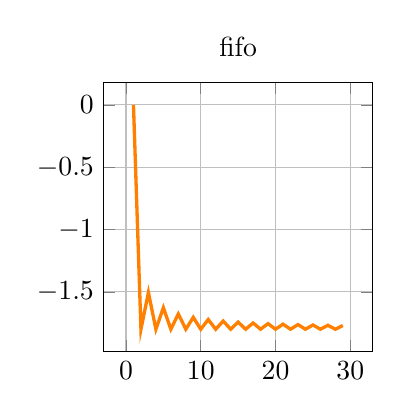
\begin{tikzpicture}
\begin{axis}[title=fifo, height=5cm, width=5cm, grid=major, xmin=({-}3.0), xmax=(33.0), ymin=({-}1.9793), ymax=(0.1799)]
\addplot[very thick,color=orange] coordinates {
(1,0.0)
(2,-1.7993405494535817)
(3,-1.505149978319906)
(4,-1.7993405494535817)
(5,-1.6266824662362944)
(6,-1.7993405494535817)
(7,-1.6766936096248666)
(8,-1.7993405494535817)
(9,-1.704150516839799)
(10,-1.7993405494535817)
(11,-1.7215358322347603)
(12,-1.7993405494535817)
(13,-1.7335411699538155)
(14,-1.7993405494535817)
(15,-1.7423322823571483)
(16,-1.7993405494535817)
(17,-1.7490488686793366)
(18,-1.7993405494535817)
(19,-1.7543483357110188)
(20,-1.7993405494535817)
(21,-1.7586366740859092)
(22,-1.7993405494535817)
(23,-1.7621782244072302)
(24,-1.7993405494535817)
(25,-1.765152527193236)
(26,-1.7993405494535817)
(27,-1.7676858167054785)
(28,-1.7993405494535817)
(29,-1.7698694445218874)
};


\end{axis}
\end{tikzpicture}
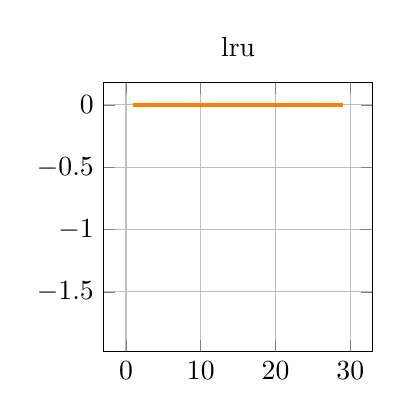
\begin{tikzpicture}
\begin{axis}[title=lru, height=5cm, width=5cm, grid=major, xmin=({-}3.0), xmax=(33.0), ymin=({-}1.9793), ymax=(0.1799)]
\addplot[very thick,color=orange] coordinates {
(1,0.0)
(2,0.0)
(3,0.0)
(4,0.0)
(5,0.0)
(6,0.0)
(7,0.0)
(8,0.0)
(9,0.0)
(10,0.0)
(11,0.0)
(12,0.0)
(13,0.0)
(14,0.0)
(15,0.0)
(16,0.0)
(17,0.0)
(18,0.0)
(19,0.0)
(20,0.0)
(21,0.0)
(22,0.0)
(23,0.0)
(24,0.0)
(25,0.0)
(26,0.0)
(27,0.0)
(28,0.0)
(29,0.0)
};


\end{axis}
\end{tikzpicture}
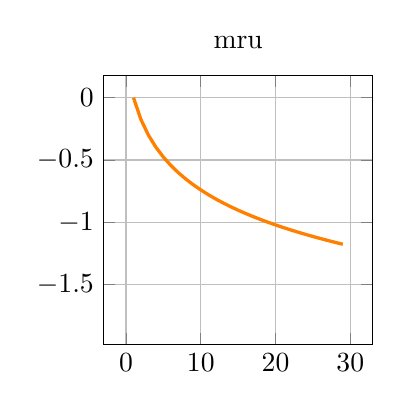
\begin{tikzpicture}
\begin{axis}[title=mru, height=5cm, width=5cm, grid=major, xmin=({-}3.0), xmax=(33.0), ymin=({-}1.9793), ymax=(0.1799)]
\addplot[very thick,color=orange] coordinates {
(1,0.0)
(2,-0.17609125905568127)
(3,-0.3010299956639812)
(4,-0.3979400086720376)
(5,-0.47712125471966244)
(6,-0.5440680443502757)
(7,-0.6020599913279624)
(8,-0.6532125137753437)
(9,-0.6989700043360187)
(10,-0.7403626894942439)
(11,-0.7781512503836436)
(12,-0.8129133566428556)
(13,-0.8450980400142568)
(14,-0.8750612633917001)
(15,-0.9030899869919435)
(16,-0.9294189257142927)
(17,-0.9542425094393249)
(18,-0.9777236052888478)
(19,-1.0)
(20,-1.021189299069938)
(21,-1.041392685158225)
(22,-1.0606978403536116)
(23,-1.0791812460476249)
(24,-1.0969100130080565)
(25,-1.1139433523068367)
(26,-1.130333768495006)
(27,-1.146128035678238)
(28,-1.1613680022349748)
(29,-1.1760912590556813)
};


\end{axis}
\end{tikzpicture}
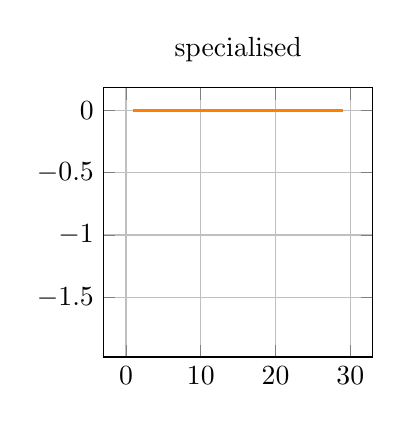
\begin{tikzpicture}
\begin{axis}[title=specialised, height=5cm, width=5cm, grid=major, xmin=({-}3.0), xmax=(33.0), ymin=({-}1.9793), ymax=(0.1799)]
\addplot[very thick,color=orange] coordinates {
(1,0.0)
(2,0.0)
(3,0.0)
(4,0.0)
(5,0.0)
(6,0.0)
(7,0.0)
(8,0.0)
(9,0.0)
(10,0.0)
(11,0.0)
(12,0.0)
(13,0.0)
(14,0.0)
(15,0.0)
(16,0.0)
(17,0.0)
(18,0.0)
(19,0.0)
(20,0.0)
(21,0.0)
(22,0.0)
(23,0.0)
(24,0.0)
(25,0.0)
(26,0.0)
(27,0.0)
(28,0.0)
(29,0.0)
};


\end{axis}
\end{tikzpicture}


\end{document}